\documentclass[aspectratio=169,11pt]{beamer}

% ================================================================
% "TABIIY TILNI QAYTA ISHLASH" KURSI
% MA'RUZA 6 --- Neyron tarmoqlarga asoslangan so'z embeddinglari: Word2Vec (CBOW)
%              (d06_word2vec.tex)
% Arxetiplar: [A][B][C][D][E] + 4 tsikl [F][G][H][I][J][K][L] +
%             [M][N][O][P][Q][R] + ilova [S]
% Rendered slayd soni: ~45 (2-haftaning ikkinchi ma'ruzasi; L1-L5 chuqurligi)
% Qulflangan [I2]: CBOW kirish = avg([0.5,0.3],[0.1,0.7]) = [0.3, 0.5]
%   --- P6 (Day 7) birinchi assert manbayi (course_map hand_example).
% ================================================================

% ================================================================
% RANGLAR  (asl fayldan o'zgarishsiz)
% ================================================================
\definecolor{cnublue}{rgb}{0.07,0.14,0.62}
\definecolor{cnubluelight}{rgb}{0.18,0.30,0.72}
\definecolor{cnubluebg}{rgb}{0.90,0.92,0.97}
\definecolor{deepblue}{rgb}{0.07,0.14,0.62}
\definecolor{deepred}{rgb}{0.60,0.00,0.00}
\definecolor{deepgreen}{rgb}{0.00,0.45,0.00}
\definecolor{halfgray}{gray}{0.55}

% ================================================================
% BEAMER MAVZU --- Boadilla + maxsus footer  (asl fayldan o'zgarishsiz)
% ================================================================
\usetheme{Boadilla}

\setbeamercolor{structure}{fg=cnublue}
\setbeamercolor{frametitle}{bg=cnublue,fg=white}
\setbeamercolor{title}{bg=cnublue,fg=white}
\setbeamercolor{block title}{bg=cnublue,fg=white}
\setbeamercolor{block body}{bg=cnubluebg,fg=black}
\setbeamercolor{alerted text}{fg=deepred}
\setbeamercolor{author in head/foot}{bg=cnubluelight,fg=white}
\setbeamercolor{section in head/foot}{bg=cnublue,fg=white}
\setbeamercolor{page number in head/foot}{bg=cnubluelight,fg=white}

\setbeamertemplate{mini frame}{}
\setbeamertemplate{mini frame in current section}{}
\setbeamertemplate{mini frame in current subsection}{}
\setbeamertemplate{headline}{}
\setbeamertemplate{navigation symbols}{}

\setbeamertemplate{footline}{%
  \leavevmode%
  \hbox{%
    \begin{beamercolorbox}[wd=0.17\paperwidth,ht=2.5ex,dp=1.25ex,leftskip=0.5em]{author in head/foot}%
      \usebeamerfont{author in head/foot}\scriptsize\insertshortauthor%
    \end{beamercolorbox}%
    \begin{beamercolorbox}[wd=0.69\paperwidth,ht=2.5ex,dp=1.25ex,center]{section in head/foot}%
      \usebeamerfont{section in head/foot}%
      \scriptsize\insertsectionnavigationhorizontal{0.69\paperwidth}{}{}%
    \end{beamercolorbox}%
    \begin{beamercolorbox}[wd=0.14\paperwidth,ht=2.5ex,dp=1.25ex,rightskip=0.5em]{page number in head/foot}%
      \hfill\scriptsize\color{white}%
      \insertframenumber{}/\inserttotalframenumber%
    \end{beamercolorbox}%
  }%
  \vskip0pt%
}

% ================================================================
% PAKETLAR  (asl fayldan o'zgarishsiz)
% ================================================================
\usepackage[utf8]{inputenc}
\usepackage[T1]{fontenc}
\usepackage{lmodern}
\usepackage{amsmath,amssymb}
\usepackage{booktabs}
\usepackage{xcolor}
\usepackage{listings}
\lstset{
    language=Python,
    basicstyle=\ttfamily\scriptsize,
    keywordstyle=\bfseries\color{deepblue},
    emphstyle=\ttfamily\color{deepred},
    stringstyle=\color{deepgreen},
    commentstyle=\itshape\color{halfgray},
    numbers=left,
    numberstyle=\scriptsize\color{halfgray},
    rulesepcolor=\color{cnublue!30},
    frame=shadowbox,
    breaklines=true,
    showstringspaces=false,
    tabsize=2
}
\usepackage{tcolorbox}
\tcbuselibrary{skins}
\tcbset{
  defbox/.style={colback=cnubluebg,colframe=cnublue,
                 fonttitle=\small\bfseries\color{white},
                 attach boxed title to top left={yshift=-2mm,xshift=4mm},
                 boxed title style={colback=cnublue,colframe=cnublue}},
  warnbox/.style={colback=orange!8,colframe=orange!70!black,
                  fonttitle=\small\bfseries},
  okbox/.style={colback=green!7,colframe=green!55!black,
                fonttitle=\small\bfseries}
}
\usepackage{tikz}
\usetikzlibrary{arrows.meta,positioning}

% ================================================================
% QO'SHIMCHALAR  (asl fayldan o'zgarishsiz)
% ================================================================
\AtBeginSection[]{%
  \begin{frame}{Prezentatsiya rejasi}
    \tableofcontents[currentsection]
  \end{frame}}

\newcommand{\bunda}[1]{{\small\textbf{bunda:}\; #1}}
\newcommand{\bajarildi}{{\color{deepgreen}\large$\checkmark$}\;}

% ================================================================
% METAMA'LUMOT
% ================================================================
\title[Word2Vec (CBOW)]{Neyron so'z embeddinglari: Word2Vec (CBOW)}
\subtitle{Tabiiy tilni qayta ishlash --- 6-ma'ruza}
\author[A.A.\,Abdulali]{A.A.\,Abdulali}
\date{23-iyun 2026}
\institute{11:00--12:20 \quad$\cdot$\quad mavzu \textnumero{}6}

% ================================================================
\begin{document}
% ================================================================

% ----------------------------------------------------------------
% [A] TITUL
% ----------------------------------------------------------------
\maketitle

% ================================================================
\section[Kirish]{Kirish: so'zlarni o'rganilgan vektorlar bilan ifodalaymiz}
% ================================================================

% ----------------------------------------------------------------
% [B] TAKRORLASH: L5 va bugungi P5
% ----------------------------------------------------------------
\begin{frame}{Takrorlash: o'tgan darsdan ikki savol}
  \begin{columns}[T]
    \begin{column}{0.49\textwidth}
      \begin{tcolorbox}[warnbox,title=1-savol]
        \small
        L5 da N-gram modeli so'zlarni \textbf{diskret} (alohida) tokenlar deb
        hisobladi: \texttt{kitob} va \texttt{kitobni} --- butunlay bog'liqsiz.
        Bu agglutinativ o'zbek tilida qanday muammoga olib keladi?
      \end{tcolorbox}
    \end{column}
    \begin{column}{0.49\textwidth}
      \begin{tcolorbox}[warnbox,title=2-savol]
        \small
        Bugun ertalab P5 da \texttt{autocomplete} \textbf{sanashga} (count)
        tayandi. Sanash ikki so'zning \textbf{ma'no o'xshashligini} o'rgata
        oladimi?
      \end{tcolorbox}
    \end{column}
  \end{columns}
  \pause
  \vspace{4pt}
  \begin{columns}[T]
    \begin{column}{0.49\textwidth}
      \begin{tcolorbox}[okbox,title=1-javob]
        \small
        \textbf{Lug'at portlaydi} (vocabulary explosion): har qo'shimchali shakl
        alohida token. Lug'at kattalashadi, sanoqlar \textbf{siyrak}lashadi.
      \end{tcolorbox}
    \end{column}
    \begin{column}{0.49\textwidth}
      \begin{tcolorbox}[okbox,title=2-javob]
        \small
        \textbf{Yo'q.} Sanash faqat ``birga uchradimi'' ni biladi; \texttt{film}
        va \texttt{kino} ni yaqin deb bilmaydi. Bugun buni \textbf{o'rganamiz}.
      \end{tcolorbox}
    \end{column}
  \end{columns}
\end{frame}

% ----------------------------------------------------------------
% [C] MAQSADLAR
% ----------------------------------------------------------------
\begin{frame}{Siz bugungi dars oxirida quyidagilarni bajara olasiz:}
  \begin{enumerate}\setlength\itemsep{6pt}
    \item \textbf{Keltirib chiqara olasiz:} nega one-hot (diskret) ifoda
          yetarli emas --- siyraklik va o'xshashlikni ko'rsata olmaslik.
    \item \textbf{Tushuntira olasiz:} CBOW arxitekturasini --- kontekst
          vektorlarini o'rtachalab markaziy so'zni bashorat qiladi
          ($\text{CBOW}_{\text{kirish}}=[0.3,0.5]$).
    \item \textbf{Hisoblay olasiz:} softmax bashorati, cross-entropy yo'qotish
          va gradientning bir qadamini qo'lda.
    \item \textbf{Baholay olasiz:} o'rganilgan embeddinglar sifatini kosinus
          o'xshashlik va analogiya orqali.
  \end{enumerate}
  \vspace{4pt}
  \begin{tcolorbox}[defbox,title=Oldindan talab]
    \footnotesize
    L3 dan: vektor, kosinus o'xshashlik. L5 dan: softmax g'oyasi yo'q edi ---
    bugun kiritamiz. Matematikadan: vektor o'rtachasi, ko'paytma, $\exp$, $\ln$,
    hosila (zanjir qoidasi).
  \end{tcolorbox}
\end{frame}

% ----------------------------------------------------------------
% [D] REJA
% ----------------------------------------------------------------
\begin{frame}{Bugungi dars rejasi:}
  \begin{center}
  \small
  \begin{tabular}{c p{5.0cm} c p{3.2cm}}
    \toprule
    \textbf{Tsikl}& \textbf{Mavzu} & \textbf{Vaqt} & \textbf{Hosil bo'luvchi natija}\\
    \midrule
    1 & Nega zich vektor? (one-hot $\to$ embedding) & 15 daq & $\cos(\text{one-hot})=0$ \\
    2 & CBOW arxitekturasi (kontekst $\to$ markaz) & 18 daq & $\text{CBOW}_{\text{kirish}}=[0.3,0.5]$ \\
    3 & O'qitish: softmax, yo'qotish, backprop & 20 daq & $\hat{y}(\text{nlp})=0.690$ \\
    4 & O'qitish jarayoni va embedding baholash & 17 daq & $\cos(\text{film},\text{kino})=0.96$ \\
    \midrule
      & Xulosa va 6-amaliyotga ko'rsatmalar & 10 daq & Ertaga nima qurishingiz \\
    \bottomrule
  \end{tabular}
  \end{center}
  \vspace{4pt}
  \begin{tcolorbox}[warnbox,title=Bu dars 2-haftani davom ettiradi]
    \footnotesize\sloppy
    Ehtimollik modellari (L5) dan \textbf{o'rganiladigan} ifodalarga o'tamiz.
    Bugungi $\text{CBOW}_{\text{kirish}}=[0.3,0.5]$ ertangi P6 da \texttt{assert} bo'ladi.
  \end{tcolorbox}
\end{frame}

% ----------------------------------------------------------------
% [E] MUAMMO BIRINCHI
% ----------------------------------------------------------------
\begin{frame}{Bugungi dars uchun muammo: ``\texttt{film}'' va ``\texttt{kino}'' yaqin ekanini qanday bilamiz?}
  \begin{columns}[T]
    \begin{column}{0.50\textwidth}
      \textbf{Sodda yechim qayerda qiynaladi:}\\[3pt]
      \small
      \begin{tcolorbox}[warnbox,title={1. One-hot: har so'z alohida o'q},top=2pt,bottom=2pt]
        \footnotesize
        \texttt{film}$=(1,0,0,\ldots)$, \texttt{kino}$=(0,1,0,\ldots)$.
        Ular \textbf{ortogonal} --- o'xshashlik $0$, garchi ma'no bir xil bo'lsa ham.
      \end{tcolorbox}
      \vspace{3pt}
      \begin{tcolorbox}[warnbox,title={2. Pretrained (L3) o'zbek uchun siyrak},top=2pt,bottom=2pt]
        \footnotesize
        P3 da ko'rdik: tayyor GloVe/Word2Vec o'zbek so'zlari uchun OOV darajasi
        baland --- coverage past.
      \end{tcolorbox}
    \end{column}
    \begin{column}{0.46\textwidth}
      \textbf{Bugungi yechim:}\\[4pt]
      \small
      \begin{enumerate}\setlength\itemsep{4pt}
        \item So'z uchun \textbf{zich} (dense), kichik o'lchamli vektor.
        \item Uni \textbf{korpusdan o'rganamiz} --- kontekstdan.
        \item Yaqin kontekstda kelgan so'zlar yaqin vektor oladi
              (\texttt{film} $\approx$ \texttt{kino}).
      \end{enumerate}
      \vspace{5pt}
      \begin{tcolorbox}[okbox,top=2pt,bottom=2pt]
        \footnotesize
        Bu g'oyaning nomi --- \textbf{Word2Vec}. Bugun uning \textbf{CBOW}
        variantini o'rganamiz.
      \end{tcolorbox}
    \end{column}
  \end{columns}
\end{frame}

% ================================================================
\section[Zich vektor]{Nega o'rganiladigan zich vektorlar?}
% ================================================================

% ----------------------------------------------------------------
% [F1] INTUITSIYA
% ----------------------------------------------------------------
\begin{frame}{Intuitsiya: so'z ma'nosi uning ``hamrohlari''da yashiringan}
  \begin{columns}[T]
    \begin{column}{0.52\textwidth}
      \small
      \textbf{Taqsimot gipotezasi} (distributional hypothesis):\\[3pt]
      \textit{``So'zni hamrohlaridan tanaymiz.''}\\[6pt]
      \texttt{film} va \texttt{kino} bir xil kontekstlarda uchraydi:\\[3pt]
      \texttt{... yaxshi \underline{\hspace{0.8cm}} ko'rdim}\\
      \texttt{... qiziq \underline{\hspace{0.8cm}} chiqdi}\\[6pt]
      Demak ularning vektorlari \textbf{yaqin} bo'lishi kerak --- agar
      vektorni kontekstdan o'rgansak.
    \end{column}
    \begin{column}{0.44\textwidth}
      \begin{tcolorbox}[okbox,top=2pt,bottom=2pt]
        \footnotesize
        One-hot da har so'z \textbf{alohida o'q} --- hech qaysi ikkitasi yaqin
        emas. Bizga \textbf{zich} fazo kerak: yaqin ma'no $\Rightarrow$ yaqin
        nuqta.
      \end{tcolorbox}
    \end{column}
  \end{columns}
\end{frame}

% ----------------------------------------------------------------
% [G1] RASMIY TA'RIF + BUNDA
% ----------------------------------------------------------------
\begin{frame}{One-hot va embedding: rasmiy ta'rif}
  \begin{tcolorbox}[defbox,title=Ta'rif: one-hot va zich embedding]
    \vspace{-0.4em}
    $$ \mathbf{x}_w \in \{0,1\}^{|V|},\quad \textstyle\sum_i x_{w,i}=1
       \qquad\Longrightarrow\qquad
       \mathbf{e}_w = W^\top \mathbf{x}_w \in \mathbb{R}^{d} $$
  \end{tcolorbox}
  \vspace{3pt}
  \bunda{$|V|$ --- lug'at hajmi; $\mathbf{x}_w$ --- $w$ so'zning one-hot vektori
  (bitta $1$, qolgani $0$); $W$ --- embedding matritsasi ($|V|\times d$);
  $d \ll |V|$ --- embedding o'lchami; $\mathbf{e}_w$ --- $w$ ning zich vektori
  (aslida $W$ ning bir qatori).}
  \vspace{5pt}
  \textbf{Asosiy farq:}
  $$ d \ll |V|: \quad |V|\!\sim\!10^5 \text{ ga qarshi } d\!\sim\!100\text{--}300 $$
  \footnotesize One-hot --- siyrak (sparse) va kontekstsiz; embedding --- zich
  (dense) va o'rganilgan.
\end{frame}

% ----------------------------------------------------------------
% [H1] KELTIRIB CHIQARISH
% ----------------------------------------------------------------
\begin{frame}{Keltirib chiqarish: nega one-hot o'xshashlikni ko'rsata olmaydi?}
  \textbf{1-qadam.} Ikki har xil so'zning one-hot vektorlari: faqat
  \emph{turli} pozitsiyada $1$ bor.
  \pause
  \textbf{2-qadam.} Ularning skalyar ko'paytmasi --- bir-biriga to'g'ri keladigan
  pozitsiya yo'q:
  $$ \mathbf{x}_a \cdot \mathbf{x}_b = \textstyle\sum_i x_{a,i}\,x_{b,i} = 0
     \quad (a \neq b) $$
  \pause
  \textbf{3-qadam.} Demak kosinus o'xshashlik ham nol:
  $$ \cos(\mathbf{x}_a,\mathbf{x}_b) = \frac{\mathbf{x}_a\cdot\mathbf{x}_b}
     {\|\mathbf{x}_a\|\,\|\mathbf{x}_b\|} = \frac{0}{1\cdot 1} = 0 $$
  \begin{tcolorbox}[okbox,top=2pt,bottom=2pt]
    \small \textbf{Xulosa:} one-hot fazoda \textbf{barcha} so'zlar bir xil
    (nol) o'xshash --- ma'no farqi yo'qoladi. Zich vektor bu muammoni hal qiladi.
  \end{tcolorbox}
\end{frame}

% ----------------------------------------------------------------
% [I1] QO'LDA MISOL
% ----------------------------------------------------------------
\begin{frame}{Qo'lda misol: one-hot o'xshashligi har doim nol}
  \begin{tcolorbox}[defbox,title={Lug'at: (film, kino, yomg'ir), |V|=3}]
    \small
    \texttt{film}$=(1,0,0)$, \quad \texttt{kino}$=(0,1,0)$, \quad
    \texttt{yomg'ir}$=(0,0,1)$.
  \end{tcolorbox}
  \vspace{0.2em}
  \begin{columns}[T]
    \begin{column}{0.52\textwidth}
      \textbf{Hisoblaymiz:}
      \begin{align*}
        \mathbf{x}_{\text{film}}\cdot\mathbf{x}_{\text{kino}}
          &= 1{\cdot}0 + 0{\cdot}1 + 0{\cdot}0 = 0\\
        \cos(\text{film},\text{kino}) &= \frac{0}{1\cdot 1} = \mathbf{0}
      \end{align*}
    \end{column}
    \begin{column}{0.44\textwidth}
      \begin{tcolorbox}[okbox,top=2pt,bottom=2pt]
        \footnotesize
        \texttt{film} va \texttt{kino} ma'noda yaqin, ammo one-hot ularni
        \texttt{film} va \texttt{yomg'ir} kabi \textbf{butunlay bog'liqsiz}
        deydi (ikkalasi ham $\cos=0$).
      \end{tcolorbox}
    \end{column}
  \end{columns}
\end{frame}

% ----------------------------------------------------------------
% [J1] SIZNING VAZIFANGIZ
% ----------------------------------------------------------------
\begin{frame}{Sizning vazifangiz: zich vektorlarda o'xshashlik}
  \begin{tcolorbox}[warnbox,title=Savol --- 90 soniya]
    \small
    Endi \textbf{o'rganilgan} zich vektorlar (dim$=2$):\\[3pt]
    $\mathbf{e}_{\text{film}}=[0.8,0.6]$, \quad $\mathbf{e}_{\text{kino}}=[0.6,0.8]$.\\[4pt]
    \textbf{\large $\cos(\text{film},\text{kino}) = ?$} \quad (har ikkala vektor uzunligi $1$)
  \end{tcolorbox}
  \pause
  \begin{tcolorbox}[okbox,title=Javob]
    \small
    $\mathbf{e}_{\text{film}}\cdot\mathbf{e}_{\text{kino}} = 0.8{\cdot}0.6 + 0.6{\cdot}0.8 = 0.48+0.48 = 0.96$\\[3pt]
    $\cos = \dfrac{0.96}{1\cdot 1} = \mathbf{0.96}$\\[3pt]
    \footnotesize One-hot da $0$ edi, zich fazoda $0.96$ --- ma'no yaqinligi
    \textbf{ko'rinadi}. Mana shuni o'rganmoqchimiz.
  \end{tcolorbox}
\end{frame}

% ----------------------------------------------------------------
% [K1] KOD <-> FORMULA  [fragile]
% ----------------------------------------------------------------
\begin{frame}[fragile]{Kod $\leftrightarrow$ formula: one-hot va embedding qidiruv}
  \begin{columns}[T]
    \begin{column}{0.56\textwidth}
\begin{lstlisting}
import numpy as np

V = ["film", "kino", "yomg'ir"]  # |V| = 3
d = 2                            # embedding o'lchami

# embedding matritsasi: |V| x d
W = np.array([[0.8, 0.6],
              [0.6, 0.8],
              [-0.6, 0.8]])

def onehot(w):
    x = np.zeros(len(V)); x[V.index(w)] = 1
    return x

# e_w = W^T x_w  ==  W ning w-qatori
e_film = W.T @ onehot("film")    # [0.8, 0.6]
print(e_film)
\end{lstlisting}
    \end{column}
    \begin{column}{0.40\textwidth}
      \textbf{Kod $\to$ formula:}\\[3pt]
      \footnotesize
      \begin{tabular}{p{2.0cm}p{2.0cm}}
        \toprule
        Kod & Formula \\
        \midrule
        \texttt{onehot(w)} & $\mathbf{x}_w$ \\
        \texttt{W} & $W$ ($|V|{\times}d$) \\
        \texttt{W.T @ x} & $W^\top\mathbf{x}_w=\mathbf{e}_w$ \\
        \bottomrule
      \end{tabular}
      \vspace{4pt}
      \begin{tcolorbox}[okbox,top=2pt,bottom=2pt]
        \footnotesize
        Amalda \texttt{W.T @ x} o'rniga shunchaki \texttt{W[index]} --- qator
        tanlanadi (matritsa ko'paytmasi shart emas).
      \end{tcolorbox}
    \end{column}
  \end{columns}
\end{frame}

% ----------------------------------------------------------------
% [L1] TUZOG'
% ----------------------------------------------------------------
\begin{frame}{Tuzoq: embedding o'zicha paydo bo'lmaydi --- uni o'rgatish kerak}
  \begin{columns}[T]
    \begin{column}{0.52\textwidth}
      \begin{tcolorbox}[warnbox,title=Tasodifiy boshlang'ich vektor ma'nosiz]
        \small
        $W$ ni tasodifiy ($\mathcal{N}(0,0.01)$) boshlaymiz. Bu paytda
        \texttt{film} va \texttt{kino} \textbf{yaqin emas} --- hali hech narsa
        o'rganilmagan.
      \end{tcolorbox}
    \end{column}
    \begin{column}{0.44\textwidth}
      \footnotesize
      Zich vektorning ``sehri'' o'z-o'zidan emas, \textbf{o'qitish} jarayonidan
      keladi.\\[4pt]
      \textbf{Savol:} $W$ ni qanday yangilaymizki, kontekstdosh so'zlar yaqin
      bo'lib qolsin? $\Rightarrow$ 2- va 3-tsikl: CBOW va backprop.
    \end{column}
  \end{columns}
\end{frame}

% ================================================================
\section[CBOW]{CBOW arxitekturasi: kontekstdan markazga}
% ================================================================

% ----------------------------------------------------------------
% [F2] INTUITSIYA
% ----------------------------------------------------------------
\begin{frame}{Intuitsiya: kontekstni o'rtachalab markaziy so'zni taxmin qilamiz}
  \begin{columns}[T]
    \begin{column}{0.52\textwidth}
      \small
      \textbf{CBOW} = \textit{Continuous Bag of Words}.\\[4pt]
      Topshiriq: atrofdagi so'zlar berilgan, \textbf{o'rtadagi} so'zni topish.\\[5pt]
      \texttt{[men, sevaman]} $\to$ \texttt{?}\\[3pt]
      Javob: \texttt{nlp} bo'lishi kerak.\\[6pt]
      \textbf{Qanday?} Kontekst so'zlarining vektorlarini \textbf{o'rtachalaymiz},
      shu o'rtacha bilan markaziy so'zni bashorat qilamiz.
    \end{column}
    \begin{column}{0.44\textwidth}
      \begin{tcolorbox}[okbox,top=2pt,bottom=2pt]
        \footnotesize
        ``Bag'' (qop) --- tartib hisobga olinmaydi: \texttt{[men, sevaman]} va
        \texttt{[sevaman, men]} bir xil o'rtacha beradi. Bu soddalashtirish ---
        CBOW ning narxi.
      \end{tcolorbox}
    \end{column}
  \end{columns}
\end{frame}

% ----------------------------------------------------------------
% [G2] RASMIY TA'RIF + BUNDA
% ----------------------------------------------------------------
\begin{frame}{CBOW arxitekturasi: rasmiy ta'rif}
  \begin{tcolorbox}[defbox,title=Ta'rif: CBOW oldinga yo'nalishi (forward)]
    \vspace{-0.4em}
    $$ \mathbf{h} = \frac{1}{2m}\sum_{j} \mathbf{e}_{c_j}, \qquad
       u_k = \mathbf{v}'_k \cdot \mathbf{h}, \qquad
       \hat{y}_k = \frac{e^{u_k}}{\sum_{k'} e^{u_{k'}}} $$
  \end{tcolorbox}
  \vspace{2pt}
  \bunda{$c_j$ --- kontekst so'zlari ($2m$ ta, oyna radiusi $m$);
  $\mathbf{e}_{c_j}$ --- ularning kirish embeddinglari; $\mathbf{h}$ ---
  \textbf{proyeksiya} (o'rtacha) qatlam; $\mathbf{v}'_k$ --- $k$ so'zning
  \textbf{chiqish} vektori ($W'$ ning ustuni); $u_k$ --- ball (score);
  $\hat{y}_k$ --- softmax bashorati.}
  \vspace{4pt}
  \footnotesize Diqqat: \textbf{ikki} matritsa bor --- kirish $W$ (embedding) va
  chiqish $W'$. Odatda embedding sifatida $W$ ishlatiladi.
\end{frame}

% ----------------------------------------------------------------
% [H2] KELTIRIB CHIQARISH
% ----------------------------------------------------------------
\begin{frame}{Keltirib chiqarish: nega kontekstni o'rtachalaymiz?}
  \textbf{1-qadam.} ``Bag'' taxmini: kontekst so'zlari --- tartibsiz to'plam,
  har biri markaziy so'zga \textbf{teng} hissa qo'shadi.
  \pause
  \textbf{2-qadam.} Teng hissa $\Rightarrow$ simmetrik birlashtirish. Yig'indi
  yoki o'rtacha bo'lishi mumkin; \textbf{o'rtacha} kontekst so'zlari soniga
  normallaydi (turli oyna o'lchamlarini solishtirsa bo'ladi):
  $$ \mathbf{h} = \frac{1}{2m}\sum_{j=1}^{2m} \mathbf{e}_{c_j} $$
  \pause
  \textbf{3-qadam.} Bu \textbf{chiziqli} amal --- nochiziqlilik (tanh,
  ReLU) \emph{yo'q}. Aynan shuning uchun proyeksiya qatlami arzon:
  $$ \mathbf{h} \;\text{hisobi} = O(2m\cdot d) \quad(\text{juda tez}) $$
  \begin{tcolorbox}[okbox,top=2pt,bottom=2pt]
    \small \textbf{Xulosa:} CBOW ``yashirin qatlam''i --- shunchaki o'rtacha.
    Soddalik $\Rightarrow$ ulkan korpusda tez o'qish (Mikolov 2013 ning maqsadi).
  \end{tcolorbox}
\end{frame}

% ----------------------------------------------------------------
% [Harch] CBOW sxemasi (TikZ)
% ----------------------------------------------------------------
\begin{frame}{CBOW oqimi: kontekst $\to$ o'rtacha $\to$ chiqish}
  \begin{center}
  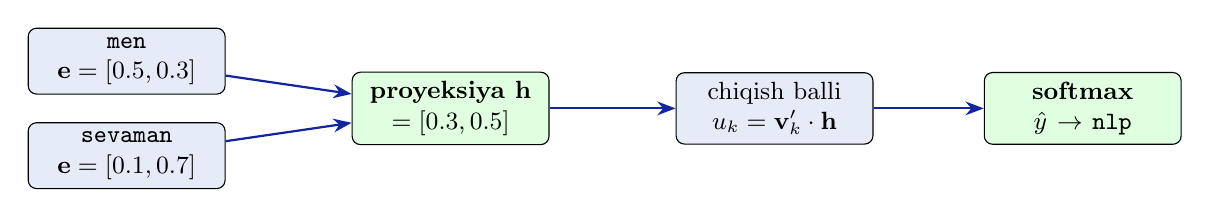
\begin{tikzpicture}[
      mod/.style={draw, fill=cnubluebg, rounded corners=3pt,
                  minimum width=2.5cm, minimum height=0.75cm,
                  font=\small, align=center},
      fin/.style={draw, fill=green!12, rounded corners=3pt,
                  minimum width=2.5cm, minimum height=0.75cm,
                  font=\small\bfseries, align=center},
      arr/.style={-{Stealth}, thick, color=cnublue}
  ]
    \node[mod] (c1) {\texttt{men}\\ $\mathbf{e}=[0.5,0.3]$};
    \node[mod, below=0.35cm of c1] (c2) {\texttt{sevaman}\\ $\mathbf{e}=[0.1,0.7]$};
    \node[fin, right=1.6cm of c1, yshift=-0.6cm] (h) {proyeksiya $\mathbf{h}$\\ $=[0.3,0.5]$};
    \node[mod, right=1.6cm of h] (u) {chiqish balli\\ $u_k=\mathbf{v}'_k\cdot\mathbf{h}$};
    \node[fin, right=1.4cm of u] (y) {softmax\\ $\hat{y}$ $\to$ \texttt{nlp}};
    \draw[arr] (c1) -- (h);
    \draw[arr] (c2) -- (h);
    \draw[arr] (h) -- (u);
    \draw[arr] (u) -- (y);
  \end{tikzpicture}
  \end{center}
  \vspace{4pt}
  \begin{tcolorbox}[okbox,top=2pt,bottom=2pt]
    \footnotesize
    Proyeksiya qatlami --- shunchaki \textbf{o'rtacha}, na'munaviy ``yashirin
    qatlam'' kabi nochiziqli emas. Aynan shu soddalik CBOW ni tez qiladi.
  \end{tcolorbox}
\end{frame}

% ----------------------------------------------------------------
% [I2] QO'LDA MISOL --- QULFLANGAN TRACEABILITY SLAYD
%
% P6 (Day 7) birinchi assert bilan solishtiring:
%   CBOW_input = avg([0.5,0.3],[0.1,0.7]) = [0.3, 0.5]   [Ma'ruza L6 [I2]-slayd]
% course_map.yaml hand_example verbatim.
% ----------------------------------------------------------------
\begin{frame}{Qo'lda misol: CBOW kirishi $=[0.3,0.5]$}
  \begin{tcolorbox}[defbox,title={Kontekst (men, sevaman); markaz nlp; dim=2}]
    \small
    $\mathbf{e}_{\text{men}}=[0.5,0.3]$, \quad
    $\mathbf{e}_{\text{sevaman}}=[0.1,0.7]$. \quad Oyna: $2m=2$ kontekst so'z.
  \end{tcolorbox}
  \vspace{0.2em}
  \begin{columns}[T]
    \begin{column}{0.52\textwidth}
      \textbf{Proyeksiya (o'rtacha):}
      \begin{align*}
        \mathbf{h} &= \tfrac{1}{2}\big(\mathbf{e}_{\text{men}}+\mathbf{e}_{\text{sevaman}}\big)\\
          &= \tfrac{1}{2}\big([0.5,0.3]+[0.1,0.7]\big)\\
          &= \tfrac{1}{2}[0.6,1.0] = \mathbf{[0.3,\,0.5]}
      \end{align*}
    \end{column}
    \begin{column}{0.44\textwidth}
      \begin{tcolorbox}[okbox,top=2pt,bottom=2pt]
        \footnotesize
        Bu $\mathbf{h}=[0.3,0.5]$ --- markaziy so'zni bashorat qilish uchun
        ishlatiladigan ``kontekst xulosasi''.
      \end{tcolorbox}
      \vspace{3pt}
      \footnotesize\color{halfgray}
      Ertangi P6 birinchi assert:\\
      \texttt{np.allclose(cbow\_input,}\\
      \texttt{\phantom{xx}[0.3, 0.5])}\\
      \textit{\# Ma'ruza L6 [I2]-slayd}
    \end{column}
  \end{columns}
\end{frame}

% ----------------------------------------------------------------
% [J2] SIZNING VAZIFANGIZ
% ----------------------------------------------------------------
\begin{frame}{Sizning vazifangiz: boshqa kontekst uchun proyeksiya}
  \begin{tcolorbox}[warnbox,title=Savol --- 90 soniya]
    \small
    Kontekst $=$ \texttt{[men, kitobni]}, dim$=2$:\\[3pt]
    $\mathbf{e}_{\text{men}}=[0.4,0.2]$, \quad $\mathbf{e}_{\text{kitobni}}=[0.2,0.6]$.\\[4pt]
    \textbf{\large $\mathbf{h} = ?$}
  \end{tcolorbox}
  \pause
  \begin{tcolorbox}[okbox,title=Javob]
    \small
    $\mathbf{h} = \tfrac{1}{2}\big([0.4,0.2]+[0.2,0.6]\big)
       = \tfrac{1}{2}[0.6,0.8] = \mathbf{[0.3,\,0.4]}$\\[3pt]
    \footnotesize Proyeksiya --- har o'lcham bo'yicha o'rtacha. Kontekst
    so'zlari soni o'zgarsa ham formula bir xil ($\tfrac{1}{2m}\sum$).
  \end{tcolorbox}
\end{frame}

% ----------------------------------------------------------------
% [K2] KOD <-> FORMULA  [fragile]
% ----------------------------------------------------------------
\begin{frame}[fragile]{Kod $\leftrightarrow$ formula: CBOW proyeksiyasi}
  \begin{columns}[T]
    \begin{column}{0.56\textwidth}
\begin{lstlisting}
import numpy as np

# kontekst so'zlarining embeddinglari
e_men     = np.array([0.5, 0.3])
e_sevaman = np.array([0.1, 0.7])

context = np.stack([e_men, e_sevaman])

# h = (1 / 2m) * sum(e_cj)
h = context.mean(axis=0)
print(h)   # [0.3 0.5]
\end{lstlisting}
    \end{column}
    \begin{column}{0.40\textwidth}
      \textbf{Kod $\to$ formula:}\\[3pt]
      \footnotesize
      \begin{tabular}{p{2.0cm}p{2.0cm}}
        \toprule
        Kod & Formula \\
        \midrule
        \texttt{np.stack} & $\{\mathbf{e}_{c_j}\}$ \\
        \texttt{.mean(axis=0)} & $\tfrac{1}{2m}\sum_j \mathbf{e}_{c_j}$ \\
        \texttt{h} & $\mathbf{h}$ \\
        \bottomrule
      \end{tabular}
      \vspace{4pt}
      \begin{tcolorbox}[okbox,top=2pt,bottom=2pt]
        \footnotesize
        Ertangi P6 da \texttt{m06 CustomWord2Vec} ichida aynan shu o'rtacha
        proyeksiya bo'ladi.
      \end{tcolorbox}
    \end{column}
  \end{columns}
\end{frame}

% ----------------------------------------------------------------
% [L2] TUZOG'
% ----------------------------------------------------------------
\begin{frame}{CBOW tuzog'i: ``bag'' tartibni unutadi}
  \begin{columns}[T]
    \begin{column}{0.52\textwidth}
      \begin{tcolorbox}[warnbox,title=Tartib yo'qoladi]
        \small
        O'rtacha kommutativ: \texttt{[men, sevaman]} va
        \texttt{[sevaman, men]} bir xil $\mathbf{h}$ beradi.\\[3pt]
        \textit{``it odamni qopdi''} va \textit{``odam itni qopdi''} ---
        CBOW uchun kontekst bir xil.
      \end{tcolorbox}
    \end{column}
    \begin{column}{0.44\textwidth}
      \footnotesize
      Bu so'z \textbf{vektorlari}ni o'rganishga ko'pincha xalal bermaydi
      (maqsad --- so'z ma'nosi, gap tahlili emas).\\[4pt]
      \textbf{Tartib muhim bo'lsa:} pozitsion kodlash, RNN (L7), Transformer
      (3-hafta) kerak bo'ladi.
    \end{column}
  \end{columns}
\end{frame}

% ================================================================
\section[O'qitish]{Neyron tarmoqni o'qitish: yo'qotish va backprop}
% ================================================================

% ----------------------------------------------------------------
% [F3] INTUITSIYA
% ----------------------------------------------------------------
\begin{frame}{Intuitsiya: xatoni o'lchaymiz, vektorlarni xato kamayadigan tomonga suramiz}
  \begin{columns}[T]
    \begin{column}{0.52\textwidth}
      \small
      O'qitish sikli (har kontekst--markaz jufti uchun):
      \begin{enumerate}\setlength\itemsep{2pt}
        \item \textbf{Forward:} $\mathbf{h}$ dan softmax bashorat $\hat{y}$.
        \item \textbf{Yo'qotish:} bashorat to'g'ri markaz so'zdan qancha uzoq?
        \item \textbf{Backward:} har vektorni xatoni kamaytiradigan tomonga
              biroz suramiz (gradient).
      \end{enumerate}
      \vspace{4pt}
      Minglab juftlar ustida takrorlasak --- kontekstdosh so'zlar yaqinlashadi.
    \end{column}
    \begin{column}{0.44\textwidth}
      \begin{tcolorbox}[okbox,top=2pt,bottom=2pt]
        \footnotesize
        ``O'rganish'' = $W$ va $W'$ ni \textbf{yangilash}. Yangilash yo'nalishi ---
        yo'qotishning gradienti (eng tik pasayish).
      \end{tcolorbox}
    \end{column}
  \end{columns}
\end{frame}

% ----------------------------------------------------------------
% [G3] RASMIY TA'RIF + BUNDA
% ----------------------------------------------------------------
\begin{frame}{Cross-entropy yo'qotish va gradient: ta'rif}
  \begin{tcolorbox}[defbox,title=Ta'rif: cross-entropy yo'qotish]
    \vspace{-0.4em}
    $$ \mathcal{L} = -\ln \hat{y}_{c} = -\ln \frac{e^{u_c}}{\sum_{k} e^{u_k}} $$
  \end{tcolorbox}
  \vspace{2pt}
  \bunda{$c$ --- haqiqiy (target) markaz so'z indeksi; $\hat{y}_c$ --- modelning
  shu so'zga bergan ehtimoli; $\mathcal{L}$ kichik $\Leftrightarrow$ model to'g'ri
  so'zga yuqori ehtimol bergan.}
  \vspace{4pt}
  \begin{tcolorbox}[defbox,title={Ta'rif: chiqish balli bo'yicha gradient}]
    \vspace{-0.4em}
    $$ \frac{\partial \mathcal{L}}{\partial u_k} = \hat{y}_k - y_k
       \qquad (\mathbf{y}\text{ --- target one-hot}) $$
  \end{tcolorbox}
  \footnotesize Bu Word2Vec ning eng nafis natijasi: gradient --- shunchaki
  \textbf{bashorat minus haqiqat}.
\end{frame}

% ----------------------------------------------------------------
% [H3] KELTIRIB CHIQARISH
% ----------------------------------------------------------------
\begin{frame}{Keltirib chiqarish: $\partial\mathcal{L}/\partial u_k = \hat{y}_k - y_k$}
  \textbf{1-qadam.} Yo'qotish: $\mathcal{L} = -u_c + \ln\sum_{k} e^{u_k}$
  (softmaxni logarifmga ochdik).
  \pause
  \textbf{2-qadam.} $u_k$ bo'yicha hosila --- ikki had:
  $$ \frac{\partial \mathcal{L}}{\partial u_k}
     = -\,\frac{\partial u_c}{\partial u_k}
       + \frac{e^{u_k}}{\sum_{k'} e^{u_{k'}}} = -y_k + \hat{y}_k $$
  \pause
  \textbf{3-qadam.} Demak ball bo'yicha gradient ($\mathbf{y}$ --- one-hot):
  $$ \frac{\partial \mathcal{L}}{\partial u_k} = \hat{y}_k - y_k $$
  \begin{tcolorbox}[okbox,top=2pt,bottom=2pt]
    \small \textbf{Xulosa:} to'g'ri so'z uchun ($y_c{=}1$) gradient
    $\hat{y}_c-1<0$ --- ballni \textbf{oshir}; boshqalar uchun $\hat{y}_k>0$ ---
    ballni \textbf{pasaytir}. Zanjir qoidasi bilan $W,W'$ ga tarqaladi.
  \end{tcolorbox}
\end{frame}

% ----------------------------------------------------------------
% [I3] QO'LDA MISOL
% ----------------------------------------------------------------
\begin{frame}{Qo'lda misol: forward, yo'qotish va gradient}
  \begin{tcolorbox}[defbox,title={h=[0.3,0.5]; nomzodlar nlp (target), kitob}]
    \scriptsize
    Chiqish vektorlari: $\mathbf{v}'_{\text{nlp}}=[1,1]$, \;
    $\mathbf{v}'_{\text{kitob}}=[0,0]$.
  \end{tcolorbox}
  \vspace{0.2em}
  \begin{columns}[T]
    \begin{column}{0.52\textwidth}
      \small\textbf{Ballar:}
      \begin{align*}
        u_{\text{nlp}} &= [1,1]\cdot[0.3,0.5] = 0.8\\
        u_{\text{kitob}} &= [0,0]\cdot[0.3,0.5] = 0
      \end{align*}
      \textbf{Softmax (target nlp):}
      \begin{align*}
        \hat{y}_{\text{nlp}} &= \frac{e^{0.8}}{e^{0.8}+e^{0}}
          = \frac{2.226}{3.226} \approx \mathbf{0.690}
      \end{align*}
    \end{column}
    \begin{column}{0.44\textwidth}
      \small\textbf{Yo'qotish:}
      $$ \mathcal{L} = -\ln 0.690 \approx \mathbf{0.371} $$
      \textbf{Gradient ($\hat{y}-y$):}
      $$ \frac{\partial\mathcal{L}}{\partial u_{\text{nlp}}} = 0.690-1 = -0.310 $$
      \begin{tcolorbox}[okbox,top=2pt,bottom=2pt]
        \footnotesize
        Manfiy $\Rightarrow$ $u_{\text{nlp}}$ ni oshirish kerak: model
        \texttt{nlp} ga \textbf{ko'proq} ehtimol bersin.
      \end{tcolorbox}
    \end{column}
  \end{columns}
\end{frame}

% ----------------------------------------------------------------
% [J3] SIZNING VAZIFANGIZ
% ----------------------------------------------------------------
\begin{frame}{Sizning vazifangiz: teng ballarda yo'qotish}
  \begin{tcolorbox}[warnbox,title=Savol --- 90 soniya]
    \small
    Agar ikkala ball ham teng bo'lsa: $u_{\text{nlp}}=0$, $u_{\text{kitob}}=0$
    (2 nomzod). Target --- \texttt{nlp}.\\[4pt]
    \textbf{\large $\hat{y}_{\text{nlp}} = ?$ \quad va \quad $\mathcal{L} = ?$}
  \end{tcolorbox}
  \pause
  \begin{tcolorbox}[okbox,title=Javob]
    \small
    $\hat{y}_{\text{nlp}} = \dfrac{e^{0}}{e^{0}+e^{0}} = \dfrac{1}{2} = \mathbf{0.5}$;
    \quad $\mathcal{L} = -\ln 0.5 \approx \mathbf{0.693}$\\[3pt]
    \footnotesize Bu --- ``hech narsa bilmaslik'' holati (tasodifiy taxmin,
    2 sinf). $0.693 = \ln 2$ --- 2 nomzodli boshlang'ich yo'qotish. O'qitish uni
    pasaytiradi.
  \end{tcolorbox}
\end{frame}

% ----------------------------------------------------------------
% [K3] KOD <-> FORMULA  [fragile]
% ----------------------------------------------------------------
\begin{frame}[fragile]{Kod $\leftrightarrow$ formula: softmax, yo'qotish, gradient}
  \begin{columns}[T]
    \begin{column}{0.58\textwidth}
\begin{lstlisting}
import numpy as np

h = np.array([0.3, 0.5])
Wout = np.array([[1, 1],    # v'_nlp
                 [0, 0]])    # v'_kitob

u = Wout @ h                 # ballar [0.8, 0.0]
yhat = np.exp(u) / np.exp(u).sum()   # softmax

y = np.array([1, 0])         # target one-hot (nlp)
loss = -np.log(yhat[0])      # 0.371
grad_u = yhat - y            # [-0.310, 0.310]

print(round(yhat[0], 3), round(loss, 3))
\end{lstlisting}
    \end{column}
    \begin{column}{0.38\textwidth}
      \textbf{Kod $\to$ formula:}\\[3pt]
      \footnotesize
      \begin{tabular}{p{1.7cm}p{1.9cm}}
        \toprule
        Kod & Formula \\
        \midrule
        \texttt{Wout @ h} & $u_k=\mathbf{v}'_k\cdot\mathbf{h}$ \\
        \texttt{exp/sum} & $\hat{y}_k$ (softmax) \\
        \texttt{-log(yhat)} & $\mathcal{L}=-\ln\hat{y}_c$ \\
        \texttt{yhat - y} & $\hat{y}_k - y_k$ \\
        \bottomrule
      \end{tabular}
      \vspace{4pt}
      \begin{tcolorbox}[warnbox,top=2pt,bottom=2pt]
        \footnotesize
        Haqiqiy Word2Vec $|V|$ katta bo'lgani uchun to'liq softmax o'rniga
        \textbf{negative sampling} ishlatadi ([L]).
      \end{tcolorbox}
    \end{column}
  \end{columns}
\end{frame}

% ----------------------------------------------------------------
% [L3] TUZOG'
% ----------------------------------------------------------------
\begin{frame}{O'qitish tuzog'i: to'liq softmax $|V|$ da juda qimmat}
  \begin{columns}[T]
    \begin{column}{0.52\textwidth}
      \begin{tcolorbox}[warnbox,title=Maxraj butun lug'at bo'ylab]
        \small
        $\hat{y}_k$ maxraji $\sum_{k'} e^{u_{k'}}$ --- har qadamda
        \textbf{butun} lug'at ($|V|\sim 10^5$) bo'yicha hisoblanadi. Bu juda
        sekin.
      \end{tcolorbox}
    \end{column}
    \begin{column}{0.44\textwidth}
      \begin{tcolorbox}[okbox,title=Yechim,top=2pt,bottom=2pt]
        \small
        \textbf{Negative sampling:} har qadamda target $+$ bir nechta tasodifiy
        ``salbiy'' so'z bilan ishlaymiz --- maxraj kichrayadi.
      \end{tcolorbox}
      \vspace{3pt}
      \footnotesize\color{halfgray}
      Muqobil: hierarchical softmax. Gensim (P6) standart sifatida negative
      sampling ishlatadi.
    \end{column}
  \end{columns}
\end{frame}

% ================================================================
\section[Baholash]{O'qitish jarayoni va embedding sifatini baholash}
% ================================================================

% ----------------------------------------------------------------
% [F4] INTUITSIYA
% ----------------------------------------------------------------
\begin{frame}{Intuitsiya: yaxshi embedding --- yaqin ma'no yaqin vektor}
  \begin{columns}[T]
    \begin{column}{0.52\textwidth}
      \small
      Korpus bo'ylab ko'p marta o'tib (epoch), $W$ ni yangilab boramiz. Sifatni
      qanday tekshiramiz?
      \begin{itemize}\setlength\itemsep{2pt}
        \item \textbf{Kosinus o'xshashlik:} sinonimlar yaqinmi?
              (\texttt{film} $\approx$ \texttt{kino})
        \item \textbf{Analogiya:} \texttt{shoh} $-$ \texttt{erkak} $+$
              \texttt{ayol} $\approx$ \texttt{malika}?
        \item \textbf{Eng o'xshashlar:} \texttt{most\_similar} mazmunlimi?
      \end{itemize}
    \end{column}
    \begin{column}{0.44\textwidth}
      \begin{tcolorbox}[okbox,top=2pt,bottom=2pt]
        \footnotesize
        Yo'qotishning pasayishi --- o'qitish ketayotganini ko'rsatadi, ammo
        \textbf{sifat} faqat shunday \emph{mazmunli} testlar bilan baholanadi.
      \end{tcolorbox}
    \end{column}
  \end{columns}
\end{frame}

% ----------------------------------------------------------------
% [G4] RASMIY TA'RIF + BUNDA
% ----------------------------------------------------------------
\begin{frame}{Kosinus o'xshashlik va analogiya: ta'rif}
  \begin{tcolorbox}[defbox,title=Ta'rif: kosinus o'xshashlik]
    \vspace{-0.4em}
    $$ \cos(\mathbf{a},\mathbf{b}) = \frac{\mathbf{a}\cdot\mathbf{b}}
       {\|\mathbf{a}\|\,\|\mathbf{b}\|} \in [-1,\,1] $$
  \end{tcolorbox}
  \vspace{2pt}
  \bunda{$\mathbf{a}\cdot\mathbf{b}$ --- skalyar ko'paytma; $\|\cdot\|$ ---
  Yevklid uzunligi; $1$ --- bir xil yo'nalish (ma'no yaqin), $0$ --- bog'liqsiz,
  $-1$ --- qarama-qarshi.}
  \vspace{4pt}
  \begin{tcolorbox}[defbox,title={Ta'rif: vektor analogiyasi}]
    \vspace{-0.4em}
    $$ \mathbf{e}_{\text{shoh}} - \mathbf{e}_{\text{erkak}}
       + \mathbf{e}_{\text{ayol}} \approx \mathbf{e}_{\text{malika}} $$
  \end{tcolorbox}
  \footnotesize Semantik munosabat (jins) vektor \emph{ayirmasi} sifatida
  saqlanadi --- L3 dagi vektor arifmetikasi.
\end{frame}

% ----------------------------------------------------------------
% [H4] KELTIRIB CHIQARISH
% ----------------------------------------------------------------
\begin{frame}{Keltirib chiqarish: nega kosinus, uzunlik emas?}
  \textbf{1-qadam.} Skalyar ko'paytma yo'nalish va uzunlikni aralashtiradi:
  $\mathbf{a}\cdot\mathbf{b} = \|\mathbf{a}\|\|\mathbf{b}\|\cos\theta$.
  \pause
  \textbf{2-qadam.} Embeddingda biz \textbf{ma'no yo'nalishi}ni qiziqtiramiz,
  uzunlikni (so'z chastotasiga bog'liq) emas.
  \pause
  \textbf{3-qadam.} Uzunlikka bo'lib, faqat yo'nalishni qoldiramiz:
  $$ \cos(\mathbf{a},\mathbf{b}) = \frac{\mathbf{a}\cdot\mathbf{b}}
     {\|\mathbf{a}\|\,\|\mathbf{b}\|} = \cos\theta $$
  \begin{tcolorbox}[okbox,top=2pt,bottom=2pt]
    \small \textbf{Xulosa:} kosinus --- ikki vektor orasidagi \textbf{burchak}.
    Shuning uchun ko'p/kam uchraydigan so'zlarni adolatli taqqoslaydi.
  \end{tcolorbox}
\end{frame}

% ----------------------------------------------------------------
% [I4] QO'LDA MISOL
% ----------------------------------------------------------------
\begin{frame}{Qo'lda misol: o'rganilgan embeddinglar sifati}
  \begin{tcolorbox}[defbox,title={O'qitishdan keyingi vektorlar (dim=2)}]
    \small
    $\mathbf{e}_{\text{film}}=[0.8,0.6]$, \quad
    $\mathbf{e}_{\text{kino}}=[0.6,0.8]$. \quad (har birining uzunligi $1$)
  \end{tcolorbox}
  \vspace{0.2em}
  \begin{columns}[T]
    \begin{column}{0.50\textwidth}
      \textbf{Hisoblaymiz:}
      \begin{align*}
        \mathbf{e}_{\text{film}}\cdot\mathbf{e}_{\text{kino}}
          &= 0.8{\cdot}0.6 + 0.6{\cdot}0.8 = 0.96\\
        \cos(\text{film},\text{kino}) &= \frac{0.96}{1\cdot 1} = \mathbf{0.96}
      \end{align*}
    \end{column}
    \begin{column}{0.46\textwidth}
      \begin{tcolorbox}[okbox,top=2pt,bottom=2pt]
        \footnotesize
        $0.96$ --- juda yuqori. Model \texttt{film} va \texttt{kino} ni
        \textbf{sinonim} sifatida o'rgangan (one-hot da bu $0$ edi --- [I1]).
        \textbf{Sifat yaxshi.}
      \end{tcolorbox}
    \end{column}
  \end{columns}
\end{frame}

% ----------------------------------------------------------------
% [J4] SIZNING VAZIFANGIZ
% ----------------------------------------------------------------
\begin{frame}{Sizning vazifangiz: bog'liqsiz juftning o'xshashligi}
  \begin{tcolorbox}[warnbox,title=Savol --- 90 soniya]
    \small
    $\mathbf{e}_{\text{film}}=[0.8,0.6]$, \quad
    $\mathbf{e}_{\text{yomg'ir}}=[-0.6,0.8]$ \; (ikkalasi uzunligi $1$):\\[4pt]
    \textbf{\large $\cos(\text{film},\text{yomg'ir}) = ?$}
  \end{tcolorbox}
  \pause
  \begin{tcolorbox}[okbox,title=Javob]
    \small
    $\mathbf{e}_{\text{film}}\cdot\mathbf{e}_{\text{yomg'ir}}
       = 0.8{\cdot}(-0.6) + 0.6{\cdot}0.8 = -0.48+0.48 = 0$\\[3pt]
    $\cos = \dfrac{0}{1\cdot 1} = \mathbf{0}$\\[3pt]
    \footnotesize Bog'liqsiz so'zlar $\Rightarrow$ $\cos \approx 0$. Model
    \texttt{film}\,$\approx$\,\texttt{kino} (0.96) ni \texttt{film}\,/\,\texttt{yomg'ir}
    (0) dan ajrata oladi --- aynan kerakli xulq.
  \end{tcolorbox}
\end{frame}

% ----------------------------------------------------------------
% [K4] KOD <-> FORMULA  [fragile]
% ----------------------------------------------------------------
\begin{frame}[fragile]{Kod $\leftrightarrow$ formula: o'xshashlik va eng o'xshashlar}
  \begin{columns}[T]
    \begin{column}{0.56\textwidth}
\begin{lstlisting}
import numpy as np

def cosine(a, b):
    return a @ b / (np.linalg.norm(a) *
                    np.linalg.norm(b))

e_film    = np.array([0.8, 0.6])
e_kino    = np.array([0.6, 0.8])
e_yomgir  = np.array([-0.6, 0.8])

print(round(cosine(e_film, e_kino), 2))   # 0.96
print(round(cosine(e_film, e_yomgir), 2)) # 0.0

# gensim: model.wv.most_similar("film")
\end{lstlisting}
    \end{column}
    \begin{column}{0.40\textwidth}
      \textbf{Kod $\to$ formula:}\\[3pt]
      \footnotesize
      \begin{tabular}{p{1.9cm}p{2.1cm}}
        \toprule
        Kod & Formula \\
        \midrule
        \texttt{a @ b} & $\mathbf{a}\cdot\mathbf{b}$ \\
        \texttt{norm(a)} & $\|\mathbf{a}\|$ \\
        \texttt{a@b/(...)} & $\cos(\mathbf{a},\mathbf{b})$ \\
        \bottomrule
      \end{tabular}
      \vspace{4pt}
      \begin{tcolorbox}[okbox,top=2pt,bottom=2pt]
        \footnotesize
        Ertangi P6 da \texttt{m06.most\_similar} aynan kosinusga tayanadi ---
        L3 dagi \texttt{m03} bilan bir xil o'lchov.
      \end{tcolorbox}
    \end{column}
  \end{columns}
\end{frame}

% ----------------------------------------------------------------
% [L4] TUZOG'
% ----------------------------------------------------------------
\begin{frame}{Baholash tuzog'i: kam ma'lumotda embedding ``shovqinli''}
  \begin{columns}[T]
    \begin{column}{0.52\textwidth}
      \begin{tcolorbox}[warnbox,title=Kam korpus = ishonchsiz vektor]
        \small
        Kam uchragan so'z (masalan 2--3 marta) yetarli kontekst ko'rmaydi ---
        uning vektori \textbf{shovqinli}, $\cos$ qiymatlari tasodifiy bo'lib
        chiqadi.
      \end{tcolorbox}
    \end{column}
    \begin{column}{0.44\textwidth}
      \footnotesize
      \textbf{Yechim:} \texttt{min\_count} bilan kam so'zlarni tashlash; korpusni
      kattalashtirish; o'zbek uchun --- stemming (m01) bilan shakllarni
      birlashtirish.\\[4pt]
      \textbf{Eslatma:} dim$=2$ misol --- pedagogik; amalda $d=100$--$300$.
    \end{column}
  \end{columns}
\end{frame}

% ================================================================
\section[Xulosa]{Xulosa va amaliyotga ko'prik}
% ================================================================

% ----------------------------------------------------------------
% [M] O'ZBEK TILIGA XOSLIK (majburiy arxetip)
% ----------------------------------------------------------------
\begin{frame}{O'zbek tilida: agglutinatsiya lug'atni portlatadi --- CBOW yordam bera oladimi?}
  \begin{columns}[T]
    \begin{column}{0.50\textwidth}
      \textbf{1. Vocabulary explosion:}\\[3pt]
      \small
      \texttt{o'rganaman}, \texttt{o'rganadi}, \texttt{o'rgandim} ---
      bir o'zak, \textbf{uch alohida} token.\\[3pt]
      \begin{tcolorbox}[warnbox,title=Oqibat,top=2pt,bottom=2pt]
        \footnotesize
        Lug'at $|V|$ portlaydi; har shakl kam uchraydi $\Rightarrow$ kam kontekst
        $\Rightarrow$ shovqinli vektor (4-tsikl [L]).
      \end{tcolorbox}
    \end{column}
    \begin{column}{0.46\textwidth}
      \textbf{2. CBOW qisman yordam beradi:}\\[3pt]
      \small
      Bu shakllar \textbf{o'xshash kontekstlarda} keladi $\Rightarrow$ CBOW
      ularga \textbf{yaqin} vektorlar berishi mumkin.\\[4pt]
      \begin{tcolorbox}[okbox,title=Lekin to'liq emas,top=2pt,bottom=2pt]
        \footnotesize
        CBOW so'zni \textbf{bo'linmas} deb biladi --- o'zak umumiyligini
        ko'rmaydi. To'liq yechim: \textbf{subword} (FastText) --- keyingi
        mavzular.
      \end{tcolorbox}
      \vspace{2pt}
      \footnotesize\textbf{Bugungi amaliy:} m01 stemming CBOW dan oldin lug'atni kichraytiradi.
    \end{column}
  \end{columns}
\end{frame}

% ----------------------------------------------------------------
% [N] SINTEZ
% ----------------------------------------------------------------
\begin{frame}{Sintez: so'z ifodalari --- siyrakdan zich, o'rganilganga}
  \begin{center}\small
  \begin{tabular}{p{2.4cm}p{2.0cm}p{2.4cm}p{3.0cm}}
    \toprule
    \textbf{Ifoda} & \textbf{O'lcham} & \textbf{O'xshashlik} & \textbf{Izoh} \\
    \midrule
    One-hot & $|V|$ (katta) & yo'q ($\cos{=}0$) & siyrak, kontekstsiz \\
    TF-IDF (L1) & $|V|$ & qisman & hujjat-darajali, siyrak \\
    Pretrained (L3) & $d$ (kichik) & bor & tayyor; o'zbek coverage past \\
    \textbf{CBOW (bugun)} & $d$ (kichik) & \textbf{bor} & \textbf{korpusdan o'rganilgan} \\
    \bottomrule
  \end{tabular}
  \end{center}
  \vspace{4pt}
  \begin{tcolorbox}[okbox,title=Asosiy g'oya,top=2pt,bottom=2pt]
    \footnotesize
    CBOW: \textbf{kontekstni o'rtachalab} markazni bashorat qiladi; xato
    ($\hat{y}-y$) vektorlarni yangilaydi; natijada \textbf{yaqin ma'no
    $\to$ yaqin vektor}. Bu --- o'z korpusingizda o'rganiladigan zich ifoda.
  \end{tcolorbox}
\end{frame}

% ----------------------------------------------------------------
% [O] SEMINAL MANBA + MUHOKAMA SAVOLI
% ----------------------------------------------------------------
\begin{frame}{Seminal manba: Mikolov va boshqalar (2013)}
  \begin{tcolorbox}[defbox,title=Manba]
    \small
    Mikolov, T., Chen, K., Corrado, G., Dean, J.\ (2013). \textbf{Efficient
    Estimation of Word Representations in Vector Space.} \textit{ICLR 2013
    (Workshop Track).}
  \end{tcolorbox}
  \vspace{5pt}
  \textbf{Ahamiyati:}
  \begin{itemize}\small\setlength\itemsep{3pt}
    \item \textbf{Word2Vec} ni kiritdi --- CBOW va Skip-gram (40\,000+ iqtibos).
    \item Sodda, sayoz model --- ulkan korpusda tez o'qiydi.
    \item Vektor arifmetikasi: \texttt{shoh}$-$\texttt{erkak}$+$\texttt{ayol}$\approx$\texttt{malika}.
  \end{itemize}
  \vspace{5pt}
  \begin{tcolorbox}[warnbox,title=Muhokama savoli (P6 gacha o'ylang)]
    \small
    CBOW kontekstdan markazni, Skip-gram markazdan kontekstni bashorat qiladi.
    \textbf{Kam ma'lumotli} o'zbek korpusi uchun qaysi biri afzalroq bo'lishi
    mumkin --- nega?
  \end{tcolorbox}
\end{frame}

% ----------------------------------------------------------------
% [P] MAQSADLAR BAJARILDI
% ----------------------------------------------------------------
\begin{frame}{Bugungi maqsadlar bajarildi}
  \begin{enumerate}\setlength\itemsep{7pt}
    \item \bajarildi \textbf{Keltirib chiqardik:} nega one-hot yetarli emas ---
          $\cos(\text{film},\text{kino})=0$ (o'xshashlik yo'qoladi).
    \item \bajarildi \textbf{Tushuntirdik:} CBOW arxitekturasi ---
          $\text{CBOW}_{\text{kirish}}=[0.3,0.5]$ (kontekst o'rtachasi).
    \item \bajarildi \textbf{Hisobladik:} softmax $\hat{y}(\text{nlp})=0.690$,
          yo'qotish $0.371$, gradient $\hat{y}-y$.
    \item \bajarildi \textbf{Baholadik:} o'rganilgan embedding ---
          $\cos(\text{film},\text{kino})=0.96$.
  \end{enumerate}
\end{frame}

% ----------------------------------------------------------------
% [Q] KO'PRIK: ERTAGA P6
% ----------------------------------------------------------------
\begin{frame}{Ertaga P6: o'zbek korpusida CBOW ni noldan o'qitamiz}
  \begin{center}
  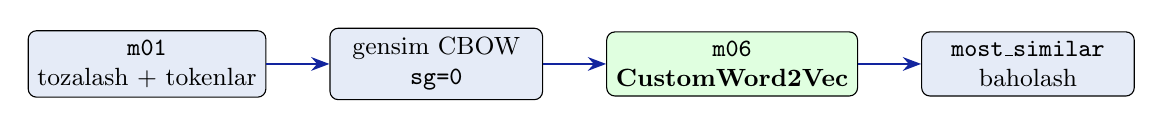
\begin{tikzpicture}[
      mod/.style={draw, fill=cnubluebg, rounded corners=3pt,
                  minimum width=2.7cm, minimum height=0.75cm,
                  font=\small, align=center},
      fin/.style={draw, fill=green!12, rounded corners=3pt,
                  minimum width=2.7cm, minimum height=0.75cm,
                  font=\small\bfseries, align=center},
      arr/.style={-{Stealth}, thick, color=cnublue}
  ]
    \node[mod] (cl) {\texttt{m01}\\ tozalash + tokenlar};
    \node[mod, right=0.8cm of cl]  (cb) {gensim CBOW\\ \texttt{sg=0}};
    \node[fin, right=0.8cm of cb]  (mv) {\texttt{m06}\\ CustomWord2Vec};
    \node[mod, right=0.8cm of mv]  (ev) {\texttt{most\_similar}\\ baholash};
    \draw[arr] (cl)--(cb);
    \draw[arr] (cb)--(mv);
    \draw[arr] (mv)--(ev);
  \end{tikzpicture}
  \end{center}
  \vspace{5pt}
  \begin{columns}[T]
    \begin{column}{0.50\textwidth}
      \textbf{P6 da qurasiz:}\\[3pt]
      \small
      \begin{itemize}\setlength\itemsep{2pt}
        \item \texttt{m06 CustomWord2Vec}: CBOW proyeksiya + o'qitish
        \item \texttt{embed(word)}, \texttt{most\_similar}
        \item O'zbek korpusida sinonim/analogiya testi
      \end{itemize}
    \end{column}
    \begin{column}{0.46\textwidth}
      \textbf{Birinchi assert (bu slayd [I2]):}\\[4pt]
      \small\ttfamily
      assert np.allclose(\\
      \phantom{xx}cbow\_input, [0.3, 0.5])\\[4pt]
      \normalfont\footnotesize\color{halfgray}
      \textit{\# Ma'ruza L6 [I2]-slayd bilan}\\
      \textit{\# solishtiring (kontekst o'rtachasi)}
    \end{column}
  \end{columns}
\end{frame}

% ----------------------------------------------------------------
% [R] ADABIYOTLAR
% ----------------------------------------------------------------
\begin{frame}{Adabiyotlar}
  \begin{enumerate}\small\setlength\itemsep{5pt}
    \item Mikolov, T., Chen, K., Corrado, G., Dean, J.\ (2013). \textit{Efficient
          Estimation of Word Representations in Vector Space.} ICLR 2013.
    \item Mikolov, T., Sutskever, I., et al.\ (2013). \textit{Distributed
          Representations of Words and Phrases and their Compositionality.}
          NeurIPS 26. (Negative sampling.)
    \item Rong, X.\ (2014). \textit{word2vec Parameter Learning Explained.}
          arXiv:1411.2738. (Backprop batafsil keltirib chiqarish.)
    \item Jurafsky, D., Martin, J.H.\ (2023). \textit{Speech and Language
          Processing}, 3-nashr. 6-bob: Vektor semantikasi va embeddinglar.
    \item \texttt{gensim.models.Word2Vec} hujjatlari --- CBOW va Skip-gram.
  \end{enumerate}
\end{frame}

% ================================================================
% [S] ILOVALAR (appendix --- slayd soniga kirmaydi)
% ================================================================
\appendix

\begin{frame}{Ilova S1: Skip-gram --- CBOW ning teskarisi}
  \small
  CBOW kontekstdan markazni bashorat qiladi; \textbf{Skip-gram} markazdan har bir
  kontekst so'zni bashorat qiladi:
  $$ \mathcal{L}_{\text{SG}} = -\sum_{j} \ln P(c_j \mid w_{\text{markaz}}) $$
  \bunda{$w_{\text{markaz}}$ --- markaziy so'z; $c_j$ --- oyna ichidagi kontekst
  so'zlari.}
  \vspace{4pt}

  Amaliy farq: Skip-gram kam uchraydigan so'zlar va kichik korpusda ko'pincha
  yaxshiroq; CBOW tez va tez-tez uchraydigan so'zlarda silliqroq. (O ning
  muhokama savoliga ishora.)
\end{frame}

\begin{frame}{Ilova S2: negative sampling yo'qotishi}
  \small
  To'liq softmax ($|V|$ bo'yicha) o'rniga, har juft uchun target $+$ $K$ ta
  tasodifiy salbiy so'z:
  $$ \mathcal{L}_{\text{neg}} = -\ln\sigma(\mathbf{v}'_c\cdot\mathbf{h})
     -\sum_{i=1}^{K} \ln\sigma(-\mathbf{v}'_{n_i}\cdot\mathbf{h}) $$
  \bunda{$\sigma$ --- sigmoid; $c$ --- target; $n_i$ --- salbiy namunalar;
  $K\sim 5$--$20$.}
  \vspace{4pt}

  Natija: har qadam $|V|$ emas, $K{+}1$ ta hisob --- o'qitish bir necha tartibga
  tezlashadi. Gensim (P6) buni standart sifatida ishlatadi.
\end{frame}

\end{document}
